\chapter{Related Work}

\section{Background}

    \subsection{GitHub and Stack Overflow}
        % GitHub (GH) is 
    
        Stack Overflow (SO) is the most popular question answering website for software developers, providing a large amount of code snippets and free-form text on a wide variety of topics. In a recent public data dump from December 9th 2018 SO listed over 42 million posts from almost 10 million registered users. Similar to other software artifacts such as source code files and documentation, text and code snippets on SO evolve over time. An example of this is when the SO community fixes bugs in code snippets, clarifies questions and answers, and updates documentation to match new API versions.
    
    \subsection{Text Processing}
    
    \subsection{Topic Modeling}
        
        Topic modeling is a technique used in the field of text mining to discover hidden patterns in a collection of textual documents. These hidden patterns are called 'topics' and they can be modeled using distributions. A topic can be defined as a collection of co-occurring words that have been grouped together by a topic modeling algorithm.
        
        Topic models are highly popular unsupervised statistical models in machine learning, as they provide a way to find structure in unstructured textual data. The most popular use case scenarios for topic models are text clustering and information retrieval tasks, where the goal is to discover structure and extract insight from text documents. Examples of such application could be the use of topic modeling to group similar words into topics, thus forming text clusters. Another sample application could be using topic modeling to detect trends in online documents and help building a recommender system for users to find similar online content. 
        
        The most used topic modeling algorithms are Latent Dirichlet Allocation (\emph{LDA}), Latent Semantic Indexing (\emph{LSI}) and Non-Negative Matrix Factorization (\emph{NMF}). The focus of this subsection will be on \emph{LDA} models.
    
        \subsubsection{What is a LDA model?}
            
           LDA is a generative probabilistic Bayesian topic model. This means that LDA observes probability distributions in input data and generates topics based on an underlying distribution of the latent (hidden) variables. LDA being also a Bayesian model, it allows Bayesian inference methods to be performed on the model. LDA models need as input a collection of documents in the form of a \emph{Document-Term Matrix} containing the number of occurrences of each word $j$ in each document $i$, and a few hyper-parameters. 
           
           LDA models come with assumptions. The first assumption is that each input document has multiple topics. This is also referred to as mixtures of topics. Furthermore, each document can be modeled as a discrete probability distribution over some number of latent (hidden) topics. The second assumption is that a topic is a collection of words with a discrete probability distribution over all unique words contained in the input documents, which is also referred to as a vocabulary of words. Lastly, the third assumption is that the number of topics is fixed and needs to be specified by the user, as LDA models do not have the capability to infer the number of topics from the input collection of documents.
           
            A trained LDA model outputs two matrices: \emph{Topic Document Matrix} and \emph{Term Topic Matrix}. The \emph{Topic Document Matrix} contains probabilities of each document generating a specific topic. The \emph{Term Topic Matrix} contains probabilities of each topic generating a specific word from the vocabulary. These two matrices can be further processed and a transformed into a weighted list of topics representing every document. Furthermore, each topic contains a list of words, which describes the topic. Large collections of unstructured textual data can be summarized, clustered, linked and even pre-processed using a LDA model and its rich output \cite{campbell2015latent}.
        
        \subsubsection{How does a LDA model work?}
        
            Apart from input collection of documents, LDA has four parameters:
            
            \begin{enumerate}
                \item $\alpha$ represents a document’s prior topic distribution, and it is sampled randomly from a Dirichlet distribution with $\alpha$ hyper-parameter. This parameter is also referred to as the prior document-topic density. Larger values of $\alpha$ result in documents containing more topics, while smaller values of $\alpha$ result in documents containing less topics. 
                
                \item $\beta$ represents a topic’s prior word distribution, and it is sampled randomly from a Dirichlet distribution with $\beta$ hyper-parameter. This parameter is also referred to as the prior topic-word density. Larger values of $\beta$ result in topics containing a larger number of words from the corpus, while lower values of $\beta$ result in topics containing less words from the corpus.
                
                \item $K$ represents the number of topics to be extracted from the input collection of documents.
                
                \item The number of iterations represents the maximum number of iterations allowed for the LDA algorithm to convergence.
            \end{enumerate}
        
            LDA assumes that it receives a collection of $D$ documents, each of length $L_i$ as input. Being a generative probabilistic model, LDA has a generative process, which can be described in the following steps:
            
            \begin{enumerate}
                \item For each topic $k$ in \{1, ..., $K$\} draw a word distribution $\phi_k \sim Dir(\beta)$
                \item For each document $d$ in \{1, ..., $D$\} draw a topic distribution $\phi_d \sim Dir(\alpha)$
                \item For each word $i$ of document $d$ draw a topic distribution $z_{d,i} \sim Multinomial(\phi_d)$ and a word distribution $w_{d,i} \sim Multinomial(\phi_{z_{d,i}})$
            \end{enumerate}
            
            \begin{figure}[!ht]
              \centering
              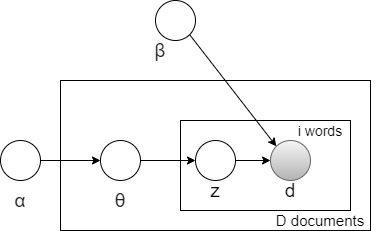
\includegraphics[width=0.7\textwidth]{figures/LDA_graphical.jpg}\\
              \caption{Graphical representation of the LDA model structure.}
              \label{fig:LDA_graph}
            \end{figure}
            
            In Figure \ref{fig:LDA_graph} the graphical representation of an LDA model is shown. As the figure shows, there are three hierarchies in the LDA model's representation. In the original LDA paper \cite{blei2003latent} the authors call these three hierarchies corpus-level, document-level and word-level representations. The hyper-parameters $\alpha$ and $\beta$ are corpus-level, as they are sampled once, when generating a text corpus based on the input documents. The latent variables $\phi_d$ are called document-level, since they get sampled once for each document. Lastly, the latent variables $z_{d,i}$ and $w_{d,i}$ are word-level, as they are  sampled only one time for each word in every document.
            
            In the training process of a LDA model the multinomial parameters $\phi_d$ for each document $d$, and $\phi_{z_{d,i}}$ for each topic are inferred. This is achieved using the \emph{Collapsed Gibbs Sampling} algorithm \cite{griffiths2004finding}. The core concept of applying \emph{Gibbs Sampling} to train the LDA model is to sequentially re-sample the posterial probability of a topic $j$ being assigned to a word $i$ of document $d$ from its conditional distribution and letting all the remaining variables stay fixed.
            
            Griffith and Steyvers \cite{griffiths2004finding} described this training process formally as Equation \ref{eq:gibbs}
            
            \begin{equation} \label{eq:gibbs}
                P(z_i = j| \textbf{$z_{-i}$}, \textbf{w}) \propto \frac{n_{-i,j}^{(w_i)} + \beta}{n_{-i,j}^{(\cdot)} + W \beta} \frac{n_{-i,j}^{(d_i)} + \alpha}{n_{-i,\cdot}^{(d_i)} + K \alpha}
            \end{equation}
            
            where $n_{-i}^{(\cdot)}$ is frequency count without counting the current assignment of $z_i$, $z_{-i}$ is $z$ without the $i$-th topic. Frequency counts in this context are the number of times a specific word was assigned to topic $j$. $K$ is the number of topics, and $W$ is the number the unique words in the text corpus. The conditional probability of topic $z_i$ being equal to topic $j$ given all other topics $z_{-i}$ and all the words $\textbf{w}$ is the full conditional distribution that gets sequentially re-sampled during the training process. The first fraction represents the proportion of assignments to topic $j$ over all documents that come from word $i$, while the second fraction represents the proportion of words in document $d$ that are currently assigned to topic $j$. In conclusion the entire training process can be summarized by the following pseudo-algorithm in Algorithm \ref{alg:training}.
            
             %1) p(topic t | document d) = the proportion of words in document d that are currently assigned to topic t, and 
            
            % 2) p(word w | topic t) = the proportion of assignments to topic t over all documents that come from this word w. 
                    
            \begin{algorithm}
                \caption{LDA Training Process using Gibbs Sampling}
                \label{alg:training}
                \begin{algorithmic}[1]
                    \REQUIRE $D$ documents, $K$ number topics, $IterNum$ - Maximum number of Gibbs Sampling iterations 
                    \FOR{each document $d$}
                        \FOR{each word $i$ in document $d$}
                            \STATE Randomly assign word $i$ to one of the $K$ topics.
                        \ENDFOR
                    \ENDFOR
                    \STATE
                    \STATE \# Perform $IterNum$ iterations of Gibbs sampling
                    \FOR{$index$ in {1, ..., $IterNum$}}
                        \FOR{each document $d$}
                            \FOR{each word $i$ in document $d$}
                                \FOR{each topic $t$ in {1, ..., K} topics}
                                    \STATE Compute full conditional probability $P$ from Equation \ref{eq:gibbs}
                                    \STATE Reassign word $i$ to topic $t$ with probability $P$
                                    \STATE \# In the LDA model $P$ is the probability that topic $t$ generated word $i$
                                \ENDFOR
                            \ENDFOR
                        \ENDFOR
                    \ENDFOR
                \end{algorithmic}
            \end{algorithm} 
                
        Note that by the reassignment in line 13 of Algorithm \ref{alg:training} it is assumed that all topic assignments except for the current word $i$ are correct, and updating the assignment of the current word using our model of how documents are generated.
        
        %After repeating the previous step a large number of times, you’ll eventually reach a roughly steady state where your assignments are pretty good. So use these assignments to estimate the topic mixtures of each document (by counting the proportion of words assigned to each topic within that document) and the words associated to each topic (by counting the proportion of words assigned to each topic overall).
        
        \subsubsection{Common Misuses and Pitfalls of LDA}
            Agrawal et al. \cite{agrawal2018wrong} examined the most common and important mis-practises of LDA in software engineering and pointed out way of correctly using LDA models. The first major mistake that the authors emphasize is the use of unstable LDA models. It is crucial to only make conclusions based on a stable LDA. Model stability in this context means that LDA needs be trained for enough Gibbs Sampling iterations that the model converges. The authors suggest that in order to achieve a stable model LDA needs to be tuned. Parameter tuning in this context refers to carefully choosing LDA's parameters based on an evaluation metric of the modeler's choice. Topics extracted from an untuned LDA model can produce unstable model output. Agrawal et al. \cite{agrawal2018wrong} work's findings state that using arbitrary chosen or default parameters for LDA models trained on software engineering data will not necessarily result in stable models and can lead to systematic errors. This finding is corroborated by Treude and Wagner \cite{treude2019predicting}, who stated that general rules of thumb for LDA parameter configuration are not applicable to textual corpora coming from software engineering domain. In their findings Agrawal et al. \cite{agrawal2018wrong} also mentions that it is not recommended to reuse an already tuned LDA model's parameters, as LDA parameter tuning is data set dependent. When performing parameter tuning, it is suggested to always re-tune the model, when training on new data.
            
            Campbell et al. \cite{campbell2015latent} writes about LDA's common pitfalls too. Topics coming out of an LDA model are independent topics generated from word distributions. The authors warn that due to the that independence of topics correlated concepts or LDA topics will not  necessarily be translated into human ideas, or even concepts. The authors also note that comparing topics by associating document contents to topics could be difficult assuming the independence between topics.
            
            Boyd-Graber et al. \cite{boyd2014care} is more concerned whether the topics extract from a topic model are interpretable, coherent, meaningful, and useful enough to a human. The authors advised to evaluate the quality of topics extracted from the following aspects: topics containing general or specific words, mixed and chained topics, identical topics, stop-words in topic, and nonsensical topics.
            
        \subsubsection{Model Selection for LDA models}
        
            According to Wallach et al. \cite{wallach2009rethinking} choosing $k$, the number of topics present in the corpus is one of the most difficult modeling decisions in topic modeling, as there are no clear methods to follow. Deciding on the right value for $k$ is very important, as according to Agrawal et al. \cite{agrawal2018wrong} this parameter matters the most for classification tasks. Choosing the number of topics $k$ could be compared to the difficult task of picking how many clusters to consider, when performing cluster analysis: there are many heuristics, but no general consensus on which one to use. For instance, Bangash et al. \cite{bangash2019developers} tried two different number of topics ($k=20$ and $k=50$) for their experiments, then picked whichever model Mallet’s optimizer\footnote{Mallet Optimizer explained: \url{https://dragonfly.hypotheses.org/1051}} returned topics that seemed close to actual topics.  Panichella et al. \cite{panichella2013effectively} designed \textit{LDA-GA}, a genetic algorithm for parameter selection for LDA. Agrawal et al. \cite{agrawal2018wrong} proposed a search-based software engineering tool to better tune the LDA model's parameters. Treude and Wagner \cite{treude2019predicting} defined the number of topics, $k$ as parameter range between 3 and 1000, then ran hyper-parameter optimization against this search space by perplexity as an evaluation metric. Hindle et al. \cite{hindle2012relating} chose the model with $k$ number of topics where the topics extracted were distinct enough. Furthermore, on top of these general rules there are many heuristics for deciding $k$ (\cite{arun2010finding}, \cite{cao2009density}, \cite{deveaud2014accurate}, \cite{griffiths2004finding}, \cite{zhao2015heuristic}).
            
            Agrawal et al. \cite{agrawal2018wrong} state that the choice of good $\alpha$ and $\beta$ hyper-parameters has the most amount of influence, when using LDA in a clustering task. Most LDA implementations recommend and use by default a fixed normalized asymmetric prior of $1.0 / topic-number$ for the $\alpha$ parameter, and a fixed prior of $0.01$ or $0.1$ for the $\beta$ parameter. Since it was shown that the use of default parameters can lead to model instability issues, hyper-parameter tuning is strongly advised in order to achieve model stability \cite{agrawal2018wrong}.
            
            %% look into further advice on how to pick parameters from the paper pdfs opened
            
        
        \subsubsection{Evaluation of LDA models}
            Boyd-Graber et al. \cite{boyd2014care} writes in their book chapter titled \textit{Care and Feeding of Topic Models: Problems, Diagnostics, and Improvements} that perplexity measurements and log-likelihood of a held-out test data are the most common evaluation methods of topic models, but they have limitations. Other forms of topic modeling evaluation could be measuring the marginal probability of a document given a topic model, but Boyd-Graber et al. \cite{boyd2014care} also say that this is not computationally feasible, since the number of possible topic assignments for words is exponential. The authors continue by stating that based on recent research perplexity does not measure the semantic coherence of topics, and good perplexity scores do not necessarily translate into good performance at some prediction based task. The same can be said for likelihood based metrics on a held-out data set, as good predictions on the held-out set do not guarantee topics with contextually accurate, semantic representation of concepts. Chang et al. \cite{chang2009reading} backs up these claims by showing that frequently predictive likelihood or perplexity based evaluation methods are not correlated, and sometimes even anti-correlated with human judgement. Furthermore, Wallach et al. \cite{wallach2009rethinking} found that perplexity and likelihood-based evaluation in most cases is less accurate than performing hyper-parameter optimization against some metric or task accuracy. This method is supported in the literature by Chen and Wang \cite{chen2011latent}, who state that a different evaluation method is to measure the LDA model's performance on one or more secondary tasks, such as some form of text classification or clustering. The authors of the original LDA paper support this method too, as Blei et al. \cite{blei2003latent} called it empirical evaluation of LDA models in various domains. 
            
            Lots of previous research was focused on designing automated measurements with as close as possible to human judgment. In 2010 this was achieved by Newman et al. \cite{newman2010visualizing}, who designed a metric based on point-wise mutual information of pairs of topic words, and called it \emph{topic coherence score}. In further research from Newman et al. \cite{newman2010visualizing},\cite{newman2010automatic} their coherence score was compared with thousands of human evaluations to conclude that their measurements mostly agree with human judgment. A year later, Mimno et al. \cite{mimno2011optimizing} corroborated that humans agree with word-pair based topic coherence. Topic coherence is further explained in a separate subsection, \ref{background:T_coherence}, where all evaluation metrics used in this project are defined. 
        
        \subsubsection{Validation of LDA models}
            Due to the various limitations and issues that some evaluation methods have, some researchers opted to manually validate the topics of LDA models by carefully reading through the collection of documents and manually checking whether the topics extracted by the model are coherent enough, and whether or not they align themselves with human judgement. 
            
            Bangash et al. \cite{bangash2019developers} performed a manual exploration of topics to validate if the LDA model's suggested topics are useful. They manually read randomly sampled documents and verified that the proper topics are assigned to the sample documents. In this case the authors also assume that their understanding is the ground truths. The down-side of such manual validation can be that it suffers from high levels of subjectivity.
            
             
            \label{topicLabeling} Bangash et al. \cite{bangash2019developers} states that ``assigning names to topics is important as LDA does not label them, and carrying out analysis on lists of words is difficult". After evaluating and picking the best model based on the above criteria, the topic labeling methodology of Bangash et al. \cite{bangash2019developers} and Hindle et al. \cite{hindle2012relating} was followed, which consisted of assigning labels to the topics based on multiple authors’ consensus. When evaluating the topics of an LDA model, it is worth noting that Hindle et al. \cite{hindle2012relating} mentioned that ``labeling some topics might not be possible, [...] as some LDA topics may not have a valid interpretation", thus some topics need to be labeled under broad terms, or be discarded.
            
            Chang et al. \cite{chang2009reading} proposed the \emph{word intrusion task} to evaluate the topics extracted from topic models. In this task a user is given six randomly ordered words. The user's job is to choose the word that does not belong. When the set of words without the word that does not belong makes sense together, the choice should be easy, while in the opposite scenario the authors observed that users tend to pick a word at random, which is a signal that the topic has low coherence. The authors also noted in their findings that there was not a clear linkage between measures of held-out set's likelihood and the measures coming from their word intrusion task.
        
        
        \subsubsection{The Use of LDA in the Software Engineering Community}
            In their book chapter on '\emph{Extracting Topics from Software Engineering Data}' Campbell et al. \cite{campbell2015latent} stated that LDA models emerged as a popular technique within the software engineering community. One reason for their popularity is that LDA models are useful for feature reduction tasks in software engineering. Another reason is that LDA models can be used to create additional features from the input documents, which then can be included in the pre-processing steps of other machine learning models. 
            
            Campbell et al. \cite{campbell2015latent} claimed that the most important use of LDA in the software engineering domain is linking software artifacts. The authors mentioned that Baldi et al. \cite{baldi2008theory} extracted LDA models' topics, then labelled and compared them to aspects in software development, concluding that some topics were mapping to actual aspects. Campbell et al. \cite{campbell2015latent} wrote that other uses of LDA models in software engineering include performing cluster analysis on issue reports and summarizing the contents of large data sets. Applying LDA to text summarization tasks requires manual or automated labelling of most topics generated by the LDA model. Hindle et al. \cite{hindle2012relating} noted that other uses of LDA in the software engineering field are in ``traceability tools, project dashboards, and knowledge management systems".
            
            % maybe include Campbell's summary paragraph
            
            % more software eng. based application.., Menzies, Treude, etc.
    
    \subsection{Evaluation Metrics Used}

        \subsubsection{Topic Coherence\label{background:T_coherence}}
        
        %% "Topic coherence metrics are motivated by measuring word association between pairs of words in the list of the top-10 most likely topic words (here, top-10 is chosen arbitrarily as the typical number of terms displayed to a user; other settings such as top-20 could work equally as well). The intuition is that a topic will likely be judged as coherent if pairs of words from that topic are associated." Boyd-Graber et al. \cite{boyd2014care}
        
        \subsubsection{Jaccard Similarity and Distance}
        
        \subsubsection{BLEU Score}
        
        \subsubsection{Cosine Similarity}

\section{Previous Work}